
% Consider a crossing $c \in \Cc(Y)$, then like when we defined the grading observe that there exists unique $c_+, c_- \in L$, such
% that $\pi(c_+) = \pi(c_-) = c$ and $z(c_+) > z(c_-)$. 

Consider a crossing $c \in \Cc(Y)$, then like when we defined the grading,
let $c_+, c_- \in L$, such $\pi(c_+) = \pi(c_-) = c$ and $z(c_+) > z(c_-)$.

\begin{defn}
Definie the the height map 
\[ H : \Cc(Y) \to  \R^+, \]
by 
$ H(c) = z(c_+) - z(c_-)$, for all $c \in \Cc$.
\end{defn}

% This lemma is needed for the proof of d^2 = 0.

\begin{lemma}
\label{prop:l_6.1}
Let $u \in W_k(Y)$. Then 
\[ \sum_{x \in Q_+} H(u(x)) - \sum_{x\in Q_-} H(u(x)) = \int_{\Pi_k} u^*(\d y \wedge \d x) > 0, \]
where $Q_+$ (resp. $Q_-$) is the set of positive (resp. negative) vertices for $u$. In particular, at least one of the vertices of $\Pi_k$ is positive.
\end{lemma}

\begin{proof}
Consider the integral $I = \int_{u(\partial \pi_k)} y \d x$. Then, by Stoke's theorem, we have
\[ I = \int_{\Pi_k} u^*(\d y \wedge \d x) > 0, \]
where the inequality is due to $u$ beeing orientation preserving.

Let $X_i \subset \partial \Pi_i$ denote the edge connection $x^k_i$ and $x^k_{i+1}$,
where $0\le i\le k-1$. Let $\gamma_i : X_i \to L$, such that 
\[ \pi \circ \gamma_i = u|_{X_i}. \] 
Since $\partial \Pi_k = \bigsqcup_i X_i$, we have 
\[ I = \sum_i \int_{\gamma_i(X_i)} y \d x. \]
Also for all $i$, $\gamma_i$ is a legendrian curve, ie. 
$\gamma_i'(d) \in \ker ( \d z - y \d x )$. So
\[ I = \sum_i \int_{\gamma_i(X_i)} \d z. \]

For each $i$, let $\sigma: [0,1] \to \R^3$ be a
parameterisation of the vertical line
segment connecting $z_+(u(x^k_i))$ with $z_-(u(^k_i))$ (ie. $\pi \circ
\sigma_i$ is constent at $u(x^k_i)$,) oriented from $z_-$ to $z_+$ if $x^k_i$ if positive for $u$ and from $z_+$ to $z_-$ if $x^k_i$ is negative for $u$. 

By assosiating $X_i$ with the unit interval, oriented from $x^k_i$ to
$x^k_{i_+1}$ we concatenate the curves into one closed curve, 
$\Gamma = \gamma_0 \star \sigma_0 \star ... \star \gamma_{k-1} \star
\sigma_{k-1}$. 
Since $\Gamma$ is closed, $\int_\Gamma \d z = 0$. Hence 
%
\[ I = \sum_i \int_{\gamma_i(X_i)} \d z - \int_\Gamma \d z = -\sum_i
\int_{\sigma{[0,1]}} \d z \quad = LHS.  \]
\end{proof}
%
The following corolary follows immideatly.
\begin{corol}
\label{prop:height_sum}
If $u \in W^+(Y)$ then $H(u(x^k_0)) \ge \sum_{i=1}^{k-1} H(u(x^k_i))$.
\end{corol}

% \begin{proof}[proof of lemma \pref{prop:W_+_finite}]
\subsubsection{proof of lemma \pref{prop:W_+_finite}}
Consider the complement of $L$ in $\R^2$. Then for some indexing set $I$, let
$\{U_i\}_{i\in I}$ denote the set of connected components, ie. $U_i$ is
connected for each $i\in I$ and 
\[ \bigcup_{i \in I} U_i = \R^2 \setminus L. \]
Since $L$ is compact, clearly $I$ is finite. Let $I = \{0,1,...,m\}$ and suppose
$U_0$ is the unbounded component.  

Let $S_i$ be the area of $U_i$, then 
\[ \int_{\Pi_k} f^*(\d y \wedge \d x) = \sum_{i=1}^n n_i(f) S_i, \] 
where the integer $n_i(f) \ge 0$ equal to the cardinality of
$f^{-1}(z)$, for $z \in U_i$.

It follows from from the corollary above that $\sum_{i=1}^m n_i(f) S_i$ is
bounded above by $\max_{c\in \Cc} H(c)$. Since $S_i > 0$, there are only finitely many
ways of choosing the coefficients $n_i$. Also, for a fixed sequence $n_1, ...,
n_m$, there are clearly only finitely many admissible immersions $f$, such that
$n_i(f) = n_i$. Hence, the total number of admissible immersions is finite.
\qed %\end{proof}

% This lemma is needed for the proof of the invariance under the Reidemeister moves
\begin{lemma}
\label{prop:deg_sum}
Let $u \in \tilde{W}_k (Y)$. Then 
\[ \sum_{x \in Q_+} \deg(u(x)) - \sum_{x \in Q_-} \deg(u(x)) = 2 - |Q_-|, \]
where $Q_+$ (resp. $Q_-$) is the set of positive (resp. negative) vertices with respect to $f$.
\end{lemma}

Note that it follows from the particular case of $|Q_+| = 1$, that the
\Ainf-maps $m_k$ has degree $2 - k$. 

\begin{proof}
Like in the proof of \pref{prop:l_6.1}, let $X_i \subset \partial \Pi_k$ be the
edge connecting $x^k_i$ and $x^k_{i+1}$. 
Consider the smooth immersions $\rho_i : X_i \to L$, such that $f|_{X_i} = \pi
\circ \rho_i$. Let $y_i = \rho_i(x^k_i)$, $y'_{i+1} = \rho_i(x^k_{i+1})$ and
$y'_0 = y'_k$, for $0 \le i \le k-1$. Then let
\[ C_1 = \sum_{i=0}^{k-1} \theta(y_i, y'_{i+1}) \qq{\text{and}}
   C_2 = \sum_{i=0}^{k-1} \theta(y'_i, y_i),  \]
where $\theta : L \times L \to \Gamma$ is the map from definition
\pref{def:theta_map}.

Then, by the additivity of $\theta$, $C_1 + C_2 = 0$ mod $m(L)$. Also $C_1 = 2 r(K)$, where $r(K)$ is the rotation
number of the closed curve $K = u(\partial \Pi_k)$ (defined as the sum of
the rotation numbers of its smooth pieces). Let $\phi_i$ denote the exterior
angle of the crossing at $u(x^k_i)$, where exterior refers to the
angle of a quadrant adjacent to the one covered by $u$, see figure
\pref{fig:outer_angle}.

\begin{figure}
\centering
% \definecolor{qqwuqq}{rgb}{.2,.2,.2}
% \definecolor{zzttqq}{rgb}{.3,.3,.3}
% \begin{tikzpicture}[line cap=round,line join=round,>=triangle 45,x=5cm,y=5cm]
% \clip(-.1,-.1) rectangle (2,2);
% \fill[line width=2pt,color=zzttqq,fill=zzttqq,fill opacity=0.1] (0,0.07) -- (0.43,0.5) -- (0,0.93) -- cycle;
% \draw [shift={(0.5,0.5)},line width=2pt,color=qqwuqq,fill=qqwuqq,fill
% opacity=0.1] (0,0) -- (45:0.427) arc (45:135:0.427) -- cycle;
% \draw [line width=2pt] (0,0)-- (1,1);
% \draw [line width=2pt] (0,1)-- (0.45,0.55);
% \draw [line width=2pt] (0.55,0.45)-- (1,0);
% \draw [line width=2pt,color=zzttqq] (0,0.07)-- (0.43,0.5);
% \draw [line width=2pt,color=zzttqq] (0.43,0.5)-- (0,0.93);
% \draw (0.014,0.6) node[anchor=north west] {$u(\Pi_k)$};
% \draw (0.449,0.856) node[anchor=north west] {$\phi_i$};
% \end{tikzpicture}
% 
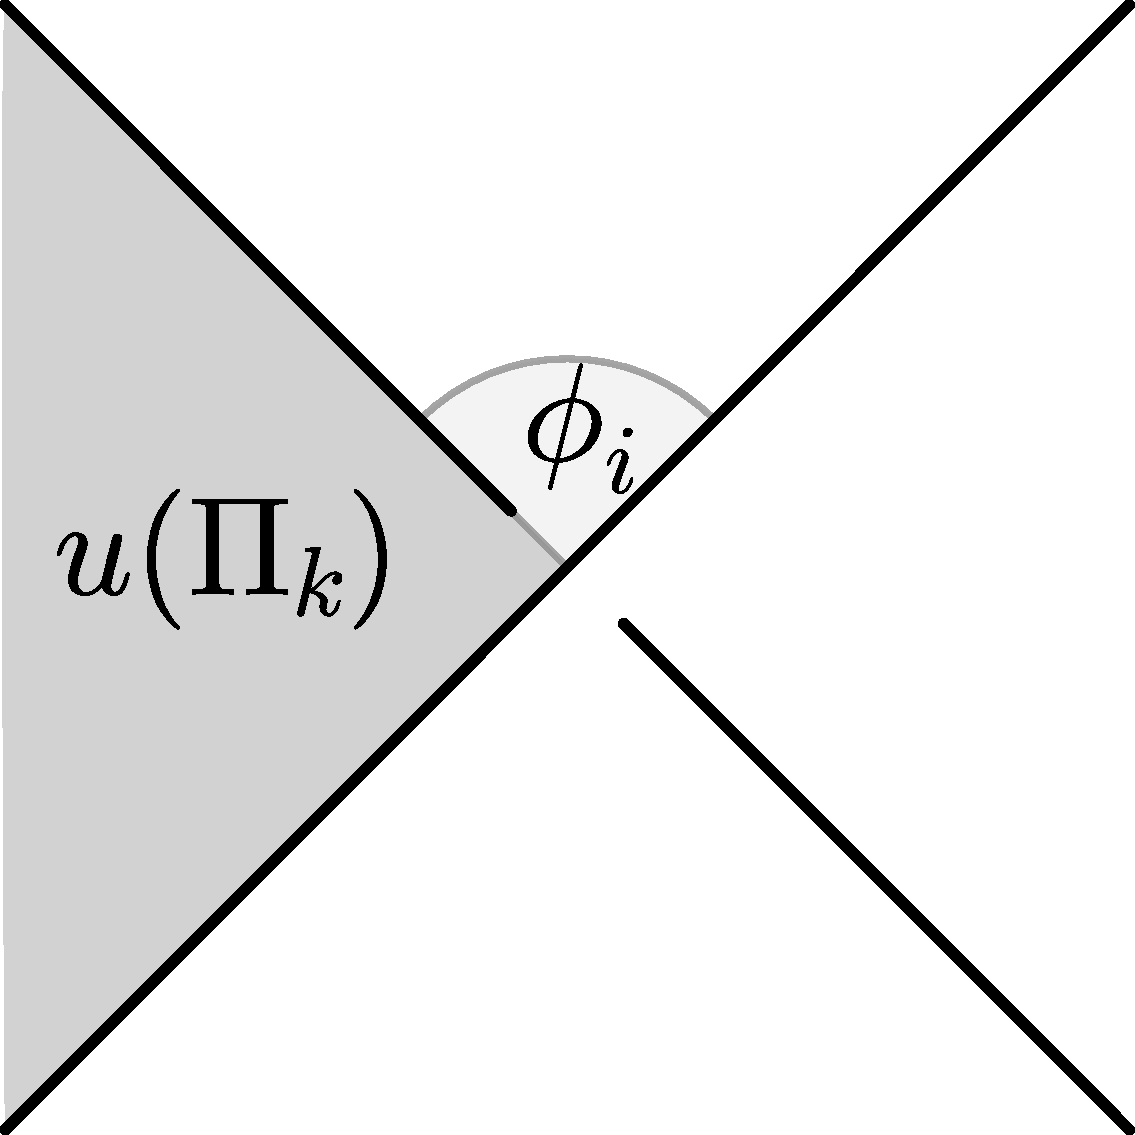
\includegraphics[width=.25\textwidth]{figs/outer_angle.pdf}
\caption{The exterior angle $\phi_i$.}
\label{fig:outer_angle}
\end{figure}

Then $r(K) = 2 - \sum \phi_i$ and thus $C_2 = -C_1 = 2\sum \phi$. Also,
\[ |u(x^k_i)| = \lceil \theta\qty(z^+_i, z^-_i) \rceil = \pwf{ - \theta_i + \phi_i  &\tif x_i  \in Q_+ \\
Q_i + (1 - \phi_) &\tif x_i \in Q_-.}  \]
By defining the sign $\mu_i$, given by $\mu_i = \mp1$ if $x_i \in Q_\pm$, we can
write 
\[ |u(x^k_i)| = \mu \theta_i - \mu_i + \frac{1+\mu_i}{2}. \]
Then, using $\mu_i^2 = 1$,
\[ LHS = - \sum \mu_i |f(x_i)| = \sum (\theta_i - \phi_i +
\frac{1+\mu_i}{2}) = -(-2 + |Q_-|).   \]

\end{proof}


